% !TEX program = xelatex
% =============================================================================
%  HSK Trainer — Technical Project Report (revised edition, November 2026)
%
%  Engine: XeLaTeX (required — uses fontspec + xeCJK for Chinese glyphs).
%  Fonts:  Latin Modern + Fandol Song (bundled with TeX Live / Overleaf).
%          Falls back to Noto Serif CJK SC when Fandol is not installed.
%
%  Compile:  xelatex report.tex  (run twice for the table of contents)
%  Overleaf: set the compiler to XeLaTeX in Menu > Settings.
% =============================================================================
\documentclass[11pt,a4paper]{article}

\usepackage[margin=2.4cm]{geometry}
\usepackage{fontspec}
\usepackage{xeCJK}
\usepackage{xcolor}
\usepackage{titlesec}
\usepackage{listings}
\usepackage{booktabs}
\usepackage{tabularx}
\usepackage{tikz}
\usepackage{enumitem}
\usepackage{caption}
\usepackage{tcolorbox}
\tcbuselibrary{skins,breakable}
\usepackage{fancyhdr}
\usepackage[hidelinks]{hyperref}

\usetikzlibrary{arrows.meta,positioning,calc,fit,backgrounds,shapes.geometric}

% ---- Fonts ------------------------------------------------------------------
% Latin Modern ships with every TeX distribution (no package install needed),
% so the report compiles out of the box locally and on Overleaf.
\setmainfont{Latin Modern Roman}
\setsansfont{Latin Modern Sans}
\setmonofont{Latin Modern Mono}[Scale=0.92]
% Fandol Song is the standard CJK font bundled with TeX Live / MiKTeX. Swap for
% "SimSun" (Windows) or "Songti SC" (macOS) if preferred.
\IfFontExistsTF{FandolSong-Regular.otf}
  {\setCJKmainfont{FandolSong-Regular.otf}[BoldFont=FandolSong-Bold.otf]}
  {\setCJKmainfont{Noto Serif CJK SC}}
\newcommand{\han}[1]{{#1}}

% ---- Palette (matches the app: cinnabar / ink / paper) ----------------------
\definecolor{cinnabar}{HTML}{C8362F}
\definecolor{ink}{HTML}{1D1A18}
\definecolor{paper}{HTML}{FBF8F3}
\definecolor{slate}{HTML}{5B5550}
\definecolor{codebg}{HTML}{F4F1EC}
\definecolor{kw}{HTML}{C8362F}
\definecolor{cmt}{HTML}{8A8178}
\definecolor{str}{HTML}{2F6F4E}

\hypersetup{
  colorlinks=true,
  linkcolor=cinnabar,
  urlcolor=cinnabar,
  citecolor=cinnabar,
  pdftitle={HSK Trainer — Technical Project Report},
  pdfauthor={Ivann Vasic}
}

% ---- Section styling --------------------------------------------------------
\titleformat{\section}
  {\sffamily\Large\bfseries\color{ink}}
  {\thesection}{0.6em}
  {}[{\color{cinnabar}\titlerule[1.2pt]}]
\titleformat{\subsection}
  {\sffamily\large\bfseries\color{cinnabar}}
  {\thesubsection}{0.5em}{}
\titlespacing*{\section}{0pt}{1.4em}{0.7em}

% ---- Headers / footers ------------------------------------------------------
\pagestyle{fancy}
\fancyhf{}
\renewcommand{\headrulewidth}{0pt}
\fancyfoot[L]{\sffamily\footnotesize\color{slate}HSK Trainer}
\fancyfoot[C]{\sffamily\footnotesize\color{slate}Technical Project Report}
\fancyfoot[R]{\sffamily\footnotesize\color{slate}\thepage}

% ---- Code listing styles ----------------------------------------------------
\lstdefinestyle{base}{
  backgroundcolor=\color{codebg},
  basicstyle=\ttfamily\footnotesize,
  keywordstyle=\color{kw}\bfseries,
  commentstyle=\color{cmt}\itshape,
  stringstyle=\color{str},
  numbers=left,
  numberstyle=\tiny\color{slate},
  numbersep=8pt,
  showstringspaces=false,
  breaklines=true,
  frame=leftline,
  framerule=2pt,
  rulecolor=\color{cinnabar},
  xleftmargin=14pt,
  framexleftmargin=10pt,
  aboveskip=10pt,belowskip=6pt,
  columns=fullflexible,
}
\lstdefinelanguage{TypeScriptX}{
  keywords={const,let,function,return,async,await,export,import,from,type,interface,if,else,for,while,new,class,extends,useState,useCallback,void,true,false,null},
  sensitive=true,
  morecomment=[l]{//},
  morecomment=[s]{/*}{*/},
  morestring=[b]",
  morestring=[b]',
  morestring=[b]`,
}
\lstset{style=base}

% ---- Callout box for architecture decisions ---------------------------------
\newtcolorbox{decision}[1]{
  enhanced, breakable,
  colback=paper, colframe=cinnabar,
  boxrule=0.6pt, arc=2pt,
  left=10pt,right=10pt,top=8pt,bottom=8pt,
  fonttitle=\sffamily\bfseries\color{ink},
  title={#1}
}

\setlist[itemize]{leftmargin=1.3em,itemsep=2pt,topsep=3pt}
\captionsetup{font=small,labelfont={sf,bf,color=cinnabar}}
\newcolumntype{L}{>{\raggedright\arraybackslash}X}

\renewcommand{\contentsname}{\sffamily Contents}

% =============================================================================
\begin{document}

% ---- Title page -------------------------------------------------------------
\begin{titlepage}
\thispagestyle{empty}
\begin{tikzpicture}[remember picture,overlay]
  \fill[ink] (current page.north west) rectangle ([yshift=-5.2cm]current page.north east);
  \node[anchor=north east,xshift=-1.6cm,yshift=-0.7cm,scale=4.4,
        text=cinnabar] at (current page.north east) {\han{学}};
  \fill[cinnabar] ([yshift=-5.2cm]current page.north west)
        rectangle ([yshift=-5.35cm]current page.north east);
\end{tikzpicture}

\vspace*{1.1cm}
\noindent{\sffamily\small\color{paper}\hspace{0.2cm}A FULL-STACK LANGUAGE-LEARNING PLATFORM}

\vspace{5.4cm}
\noindent{\sffamily\Huge\bfseries\color{ink}HSK Trainer}\\[0.35cm]
{\sffamily\large\color{slate}A complete preparation platform for the Chinese HSK exams:\\
spaced repetition (FSRS), exam-format listening and writing practice,\\
grammar, classifiers, tones, and LLM-powered correction}

\vfill
\noindent
\begin{tabular}{@{}ll@{}}
  {\sffamily\bfseries\color{ink}Author}  & Ivann Vasic \\[3pt]
  {\sffamily\bfseries\color{ink}Stack}   & FastAPI \;\textperiodcentered\; Next.js \;\textperiodcentered\; Postgres \;\textperiodcentered\; Anthropic Claude \\[3pt]
  {\sffamily\bfseries\color{ink}Type}    & Technical project report \\[3pt]
  {\sffamily\bfseries\color{ink}Edition} & Revised, November 2026 \\
\end{tabular}

\vspace{0.6cm}
\noindent{\color{cinnabar}\rule{\linewidth}{1.2pt}}
\end{titlepage}

% ---- Abstract + TOC ---------------------------------------------------------
\section*{\sffamily Abstract}
\noindent
HSK Trainer is a web application that prepares learners for the official
\emph{HSK} Chinese proficiency exams. What started as a vocabulary quiz with an
LLM grader has grown into a full preparation platform organised in eight study
areas: vocabulary review driven by a modern spaced-repetition scheduler (FSRS)
over the complete HSK~2.0 and HSK~3.0 word lists (levels 1--5, 3,600 words);
listening and writing papers that reproduce the structure of the real exams;
the 210 official grammar points of levels 1--3; measure words; tones; free
written expression corrected by Anthropic Claude over a live stream; a
handwriting pad; and a statistics dashboard. This report describes the purpose
of the system, each feature, the decoupled architecture behind it, the
engineering decisions and their trade-offs, and how the whole is tested and
deployed at near-zero cost. The project began as a single Streamlit prototype
and was deliberately rebuilt as a typed FastAPI service with a separate Next.js
front end to demonstrate production-oriented software, data and AI-integration
practices.

\vspace{0.8em}
{\footnotesize\tableofcontents}
\thispagestyle{fancy}
\newpage

% =============================================================================
\section{Introduction and Motivation}

Preparing for the HSK requires several distinct skills: \emph{recognising}
vocabulary quickly, \emph{understanding} spoken Chinese at exam speed,
\emph{producing} correct characters and sentences, and mastering the grammar
points the syllabus lists for each level. Generic flashcard apps address the
first poorly (fixed intervals, no production practice) and the others not at
all, while past papers are scarce --- especially for the new HSK~3.0 format,
whose first sessions take place in 2026.

HSK Trainer was built to solve a concrete personal need --- preparing the
HSK~3.0 level~3 exam as a French speaker --- while simultaneously serving as an
engineering portfolio piece. That dual purpose shaped every decision: features
were only kept if they passed the ``would I use this every day?'' test, and the
architecture was chosen to make production practices visible (typed APIs,
migrations, streaming LLM integration, CI, infrastructure-as-code).

The application interface is in French (the learner's language) and the
content is Chinese. It supports \textbf{both exam versions}: HSK~2.0 (2012
lists, 2,496 words for levels 1--5) and HSK~3.0 (2025 syllabus, 3,600 words for
levels 1--5). Three ideas run through the whole product:

\begin{itemize}
  \item \textbf{Schedule what is about to be forgotten.} An FSRS scheduler
        selects the vocabulary to review; every other area prioritises what has
        never been practised, then what was failed last time.
  \item \textbf{Practise in the format of the exam.} Listening and writing
        sets follow the official papers part by part, with the same number of
        questions and recordings played twice.
  \item \textbf{Use the LLM where judgement is needed, and nowhere else.}
        Claude grades free production (texts, sentences), writes example
        sentences and extends the question bank; everything that can be checked
        deterministically is checked in code.
\end{itemize}

% =============================================================================
\section{Product Overview}

After signing in, the learner navigates between eight tabs, plus an Admin page
reserved to the owner. Table~\ref{tab:areas} summarises them; the following
subsections describe each one.

\begin{table}[h]
\centering\small
\begin{tabularx}{\linewidth}{@{}llL@{}}
\toprule
\textbf{Tab} & \textbf{Skill} & \textbf{Content} \\
\midrule
Compréhension   & Vocabulary     & FSRS review of the HSK word lists, three answer modes \\
Écoute          & Listening      & Listening papers of HSK 1--3 in the real format \\
Écriture HSK    & Writing        & Writing papers of HSK 1--3, sentences graded by Claude \\
Grammaire       & Grammar        & 210 official grammar points, lessons and quizzes \\
Classificateurs & Measure words  & 44 classifiers of HSK 1--3, three exercise modes \\
Tons            & Pronunciation  & Find or dictate the tone of each syllable \\
Expression      & Free writing   & Short texts corrected by Claude over a live stream \\
Compte          & Follow-up      & Dashboard, study statistics, word lists, drawings \\
\bottomrule
\end{tabularx}
\caption{The study areas of the application.}
\label{tab:areas}
\end{table}

\subsection{Vocabulary review (Compréhension)}

The core of the app. A session is configured in a few clicks and then runs
entirely client-side for instant transitions.

\begin{itemize}
  \item \textbf{Session setup} --- one or several HSK levels mixed in the same
        session; 10, 20, 50, a custom number or the maximum available (up to
        4,000 cards); and a choice of words: \emph{all} (due cards first, with
        some new words), \emph{new only}, or \emph{revision only}.
  \item \textbf{Three answer modes} --- \emph{self-assessment} (the fastest,
        ideal on a phone); \emph{pinyin input}, where the pinyin must be typed
        before judging (tone marks are optional in the comparison); and
        \emph{hanzi input}, the reverse direction: the French translation is
        shown and the word must be typed in characters. In that last mode
        nothing that would reveal the answer --- audio, examples, drawings ---
        appears before the answer is checked.
  \item \textbf{Rating} --- four FSRS ratings (again / hard / good / easy) with
        keyboard shortcuts 1--4, progressive hints (pinyin first, then the full
        solution), and an optional \emph{pinyin lock} that keeps the pinyin
        displayed on every card, saved on the account.
  \item \textbf{Study tools on each card} --- a ``listen'' button; example
        sentences generated on demand by Claude (sentence, pinyin, translation,
        an explanation of the word and its decomposition character by
        character), saved per user and shown again at later reviews; and a
        handwriting pad.
  \item \textbf{HSK 2.0 / 3.0 switch} --- a toggle selects the exam version. A
        word is a single entry listed under one level per version, so its
        progress is shared: switching version only changes which level the
        word belongs to.
\end{itemize}

\subsection{Listening and writing in the exam format}

The \emph{Écoute} and \emph{Écriture HSK} tabs reproduce the papers of levels
1--3. For HSK~3.0 the structure follows the official 2025 specification and
sample papers; for HSK~2.0 it follows the 2012 sample papers. Each part keeps
its order, its instruction and its number of questions.

\begin{itemize}
  \item \textbf{Twelve question types} --- picture choice, picture true/false,
        picture matching, word matching, short and long dialogue questions,
        passage questions and true/false statements for listening; missing
        character from pinyin, word reordering and sentence writing for
        writing. Pictures of the real papers are replaced by short French
        descriptions of the scene.
  \item \textbf{Recordings without audio files} --- each recording is a script
        read by the device's own Chinese voices through the Web Speech API, one
        voice per speaker, played twice automatically as in the exam, with a
        ``listen again'' button.
  \item \textbf{A reviewed question bank} --- more than 330 hand-reviewed items
        (about 400 questions). A build script validates every item and checks
        that its Chinese only uses characters from the word lists of its level.
  \item \textbf{``New series'' by Claude} --- for any part, the learner can ask
        for a brand-new set. Generated items go through the same parser and the
        same vocabulary check as the bank, and are kept for that learner.
  \item \textbf{Scores} --- every finished set is saved, and the catalogue of
        parts shows the number of attempts and the best and latest scores.
\end{itemize}

\paragraph{Sentence writing (HSK~3, writing part~2).} This part of the exam
asks for a sentence built around an imposed word. The app turns it into a
personalised drill with three sources: \emph{words already seen} in the
learner's own reviews, \emph{weak words} (up to fifty words whose mastery score
is below one half), and \emph{grammar structures} --- 61 major structures of
levels~2--3 such as the \han{把} construction or \han{越来越}. Structures never
practised come first, then those failed last time. Claude grades each sentence
(correctness, corrected version with pinyin and translation, a short
explanation and a model sentence when wrong); for structures, the pattern is
only revealed in the correction. A hint with the meaning is available on
demand, and a \emph{skip} button replaces the current item: a skipped structure
is counted as mastered and goes to the back of the queue without affecting
scores, while a skipped word is simply replaced.

\subsection{Grammar}

The 210 official grammar points of levels 1--3 (48 + 81 + 81, from the
\han{语法等级大纲} of the 2021 standards) each have a card written for this app: a
French title, an explanation, the pattern, examples, and a short quiz. The
learner can practise one point or a mixed quiz, and progress is tracked per
point.

\subsection{Classifiers}

Measure words are a classic difficulty for French speakers. The tab covers 44
nominal and verbal classifiers of HSK 1--3, each with a reference card (usage,
typical nouns, examples, common traps) and 178 reviewed fill-in sentences whose
distractors are unambiguously wrong. Three modes exist: choosing the classifier
among options, \emph{writing} it with no options, and a quiz on what each
classifier is used for. Claude can generate ten more sentences for a classifier
on request.

\subsection{Tones}

The \emph{Tons} tab drills the tone of every syllable of the HSK words of the
chosen levels. In the first mode the word is displayed and the learner picks
the tone (1--4 or neutral) of each character; a dictation mode plays the word
instead of showing its pinyin. The split of a word's pinyin into syllables is
computed in the browser with \texttt{pinyin-pro}; no server call is needed
beyond loading the word list.

\subsection{Free written expression}

The learner picks a curated subject, asks Claude for a new one, or writes their
own, then submits a short text in Chinese. The correction streams back in real
time: a score, the corrected version with pinyin and translation, a typed list
of mistakes, strengths and a recommendation. A closing feedback loop ties this
area to vocabulary: the words Claude flags as misused are automatically pushed
back into the FSRS review queue. Past attempts remain browsable.

\subsection{Handwriting practice}

``S'entraîner à écrire'' opens one \han{米字格} practice square per character of
the word. The pad is stylus-friendly (palm rejection, pen, eraser, undo,
clear). Strokes are kept as vectors normalised to their cell, so the pad can be
resized without loss and the drawing is exported as a clean fixed-resolution
PNG. Drawings are saved per user and per word, shown again at later reviews and
gathered in a gallery on the account page.

\subsection{Dashboard and statistics}

The account page answers two questions: \emph{where am I?} and \emph{am I
working regularly?}

\begin{itemize}
  \item \textbf{Progress} --- key figures (streak, success rate, words seen and
        mastered), progress per HSK level, a mastery-distribution chart, a
        forecast of upcoming reviews, and browsable lists of \emph{mastered},
        \emph{known} and \emph{to-review} words.
  \item \textbf{Activity} --- a 90-day heatmap, the number of new words seen
        per day, and quiz and expression progression curves.
  \item \textbf{Study statistics} --- over 7, 30 or 90 days: activity per tab,
        vocabulary growth, time spent, and habits by hour and weekday.
\end{itemize}

All days follow the learner's own clock: the browser sends its time zone in an
\texttt{X-Timezone} header, so a review done at 07:00 in Shanghai is not
attributed to the previous day by a server running in UTC.

\subsection{Administration and usage limits}

A read-only \emph{Admin} page, visible only to the accounts whose e-mail is
listed in an environment variable, shows site-wide figures (accounts, sign-ups
per week, active users, Claude token consumption) and, for each account,
activity counters and the same statistics page the user sees. It deliberately
exposes counters and dates only: no password hash, no text written by users, no
drawings.

Every call to Claude is metered. Each of the five kinds of call (text
correction, subject generation, example generation, exercise generation,
sentence grading) is limited to 15 per user per day, and to 100 for
administrators. Registration can also be restricted to an allow-list of
e-mails.

% =============================================================================
\section{Architecture}

The system is a \textbf{monorepo} with two independently deployable services
that communicate over HTTPS using JSON and, for the text-correction endpoint, a
Server-Sent-Events (SSE) stream.

\begin{figure}[h]
\centering
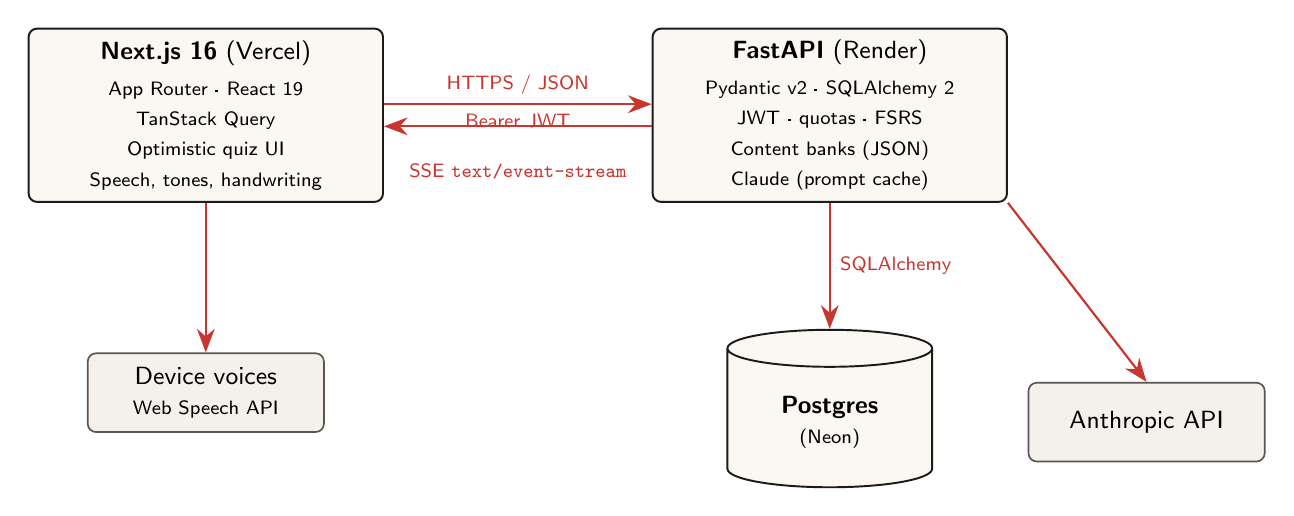
\begin{tikzpicture}[
  font=\sffamily\small,
  box/.style={rectangle,rounded corners=3pt,draw=ink,line width=0.7pt,
    fill=paper,minimum width=4.5cm,minimum height=2.2cm,align=center},
  ext/.style={rectangle,rounded corners=3pt,draw=slate,line width=0.6pt,
    fill=codebg,minimum width=3.0cm,minimum height=1.0cm,align=center},
  db/.style={cylinder,shape border rotate=90,aspect=0.32,draw=ink,
    line width=0.7pt,fill=paper,minimum width=2.6cm,minimum height=2.0cm,
    align=center},
  arr/.style={-{Stealth[length=3mm]},line width=0.8pt,color=cinnabar}
]
  \node[box] (fe) {\textbf{Next.js 16} (Vercel)\\[2pt]
    \scriptsize App Router \textperiodcentered\ React 19\\
    \scriptsize TanStack Query\\ \scriptsize Optimistic quiz UI\\
    \scriptsize Speech, tones, handwriting};
  \node[box,right=3.4cm of fe] (be) {\textbf{FastAPI} (Render)\\[2pt]
    \scriptsize Pydantic v2 \textperiodcentered\ SQLAlchemy 2\\
    \scriptsize JWT \textperiodcentered\ quotas \textperiodcentered\ FSRS\\
    \scriptsize Content banks (JSON)\\
    \scriptsize Claude (prompt cache)};
  \node[db,below=1.6cm of be] (pg) {\textbf{Postgres}\\\scriptsize (Neon)};
  \node[ext,below=1.9cm of fe] (tts) {Device voices\\\scriptsize Web Speech API};
  \node[ext,right=1.2cm of pg] (claude) {Anthropic API};

  \draw[arr] ([yshift=4pt]fe.east) -- node[above,font=\scriptsize\sffamily]
    {HTTPS / JSON} node[below,font=\scriptsize\sffamily]{Bearer JWT}
    ([yshift=4pt]be.west);
  \draw[arr] ([yshift=-4pt]be.west) -- node[below,font=\scriptsize\sffamily,
    yshift=-10pt]{SSE \texttt{text/event-stream}} ([yshift=-4pt]fe.east);
  \draw[arr] (be.south) -- node[right,font=\scriptsize\sffamily]
    {SQLAlchemy} (pg.north);
  \draw[arr] (fe.south) -- (tts.north);
  \draw[arr] (be.south east) -- (claude.north);
\end{tikzpicture}
\caption{High-level service topology. The front end and back end deploy
independently; speech synthesis happens entirely on the learner's device.}
\end{figure}

\noindent The repository layout reflects this separation:

\begin{lstlisting}[language=,numbers=none]
backend/    FastAPI service (Python 3.12)
  app/api/v1/      auth, quizzes, srs, mastery, examples, drawings, exercises,
                   classifiers, expression, account, admin
  app/services/    srs, llm, exercise, grammar, classifier, expression, stats,
                   account, admin, version, drawing, example, ...
  app/models/      SQLAlchemy ORM (13 tables)
  app/schemas/     Pydantic v2 request/response models
  app/core/        settings, security (JWT, password hashing), time zones
  alembic/         8 migrations (0001 baseline -> 0008 exercises)
  data/            word lists (HSK 2.0 and 3.0), exercise bank, grammar points,
                   classifiers, structures, writing subjects
  scripts/         build + validation scripts for the content banks
  tests/           pytest, 138 tests (Anthropic mocked)
frontend/   Next.js 16 app (TypeScript)
  app/             routes: landing, signin/signup, comprehension, listening,
                   writing, grammar, classifiers, tones, expression, account, admin
  components/      quiz, exercises, grammar, classifiers, tones, expression,
                   writing (drawing pad), dashboard, charts, admin, ui
  lib/             typed API client, auth context, SSE consumer, speech,
                   tones, handwriting, pinyin helpers
  tests/           Vitest + Testing Library, 87 tests
\end{lstlisting}

\subsection{Request lifecycle}

Every authenticated request carries a JSON Web Token in an
\texttt{Authorization: Bearer} header. A reusable FastAPI dependency decodes
and validates it, resolves the user, and --- on the endpoints that call Claude
--- enforces the per-user daily limit before the handler runs. Admin endpoints
add a second dependency that returns 403 to everybody else.

\begin{figure}[h]
\centering
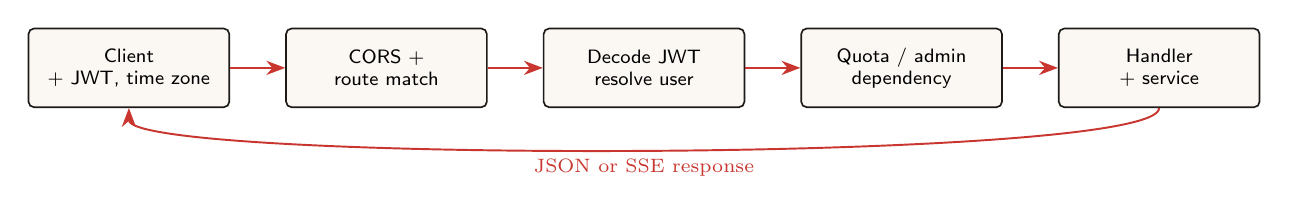
\begin{tikzpicture}[
  font=\sffamily\scriptsize,
  stage/.style={rectangle,rounded corners=2pt,draw=ink,line width=0.6pt,
    fill=paper,minimum height=1.0cm,minimum width=2.55cm,align=center},
  arr/.style={-{Stealth[length=2.4mm]},line width=0.7pt,color=cinnabar}
]
  \node[stage] (a) {Client\\\scriptsize+ JWT, time zone};
  \node[stage,right=0.7cm of a] (b) {CORS +\\route match};
  \node[stage,right=0.7cm of b] (c) {Decode JWT\\resolve user};
  \node[stage,right=0.7cm of c] (d) {Quota / admin\\dependency};
  \node[stage,right=0.7cm of d] (e) {Handler\\+ service};
  \draw[arr] (a)--(b); \draw[arr] (b)--(c); \draw[arr] (c)--(d);
  \draw[arr] (d)--(e);
  \draw[arr] (e.south) .. controls +(0,-0.7) and +(0,-0.7) ..
    node[below,font=\scriptsize]{JSON or SSE response} (a.south);
\end{tikzpicture}
\caption{Request pipeline. Auth, quotas and admin rights are dependencies, so
handlers stay free of cross-cutting concerns.}
\end{figure}

% =============================================================================
\section{Technology Stack}

\begin{table}[h]
\centering\small
\begin{tabularx}{\linewidth}{@{}llL@{}}
\toprule
\textbf{Layer} & \textbf{Choice} & \textbf{Rationale} \\
\midrule
API            & FastAPI + Pydantic v2   & Typed I/O, auto OpenAPI, SSE streaming \\
ORM            & SQLAlchemy 2.x          & Mature, explicit, Postgres + SQLite \\
Migrations     & Alembic                 & Versioned schema, idempotent migrations run at deploy \\
Auth           & JWT (HS256) + PBKDF2    & Stateless, no session store \\
Scheduler      & FSRS (py-fsrs 6)        & ML-based, outperforms SM-2 \\
LLM            & Claude Haiku 4.5        & Cheap, fast, prompt-cache friendly \\
Content        & YAML sources $\to$ JSON & Reviewed by hand, validated by build scripts \\
Front end      & Next.js 16 / React 19   & App Router, mature ecosystem \\
Server state   & TanStack Query          & Caching, retries, optimistic updates \\
Styling        & Tailwind v4             & CSS-first tokens, light and dark themes \\
Forms          & react-hook-form + zod   & Typed validation \\
Charts         & Recharts                & Composable charts for the dashboard \\
Animation      & Framer Motion           & Card transitions \\
Speech         & Web Speech API          & Free, on-device Chinese voices, works offline \\
Pinyin         & pinyin-pro              & Syllable splitting for the tone drills \\
Database       & Postgres (Neon)         & Free tier, autosuspend, branching \\
Tests          & pytest, Vitest          & Offline suites, Testing Library for components \\
CI             & GitHub Actions          & pytest + Vitest + production build \\
\bottomrule
\end{tabularx}
\caption{Stack and the reasoning behind each layer.}
\end{table}

% =============================================================================
\section{Backend Design}

\subsection{API surface}

The API is versioned under \texttt{/v1} and fully described by an
auto-generated OpenAPI document (Swagger UI at \texttt{/docs}).

\begin{table}[h]
\centering\small
\begin{tabularx}{\linewidth}{@{}lL@{}}
\toprule
\textbf{Group} & \textbf{Endpoints} \\
\midrule
\texttt{auth}        & register, login, me (with the computed admin flag) \\
\texttt{quizzes}     & catalogue of levels per HSK version, entries of a level \\
\texttt{srs}         & rate a card, fetch a session (due / new / revision), counters \\
\texttt{mastery}     & per-word state for the word lists \\
\texttt{examples}    & list and generate example sentences for a word \\
\texttt{drawings}    & save, list, delete handwriting drawings; gallery \\
\texttt{exercises}   & catalogue of parts, practice set, results, generation by Claude,
                       sentence and structure grading, skip, grammar points \\
\texttt{classifiers} & reference cards, quiz (three modes), sentence generation \\
\texttt{expression}  & subjects, subject generation, streamed correction, attempts, quota \\
\texttt{account}     & dashboard overview, study statistics, settings (version, pinyin lock) \\
\texttt{admin}       & accounts overview and per-account statistics (read-only) \\
\bottomrule
\end{tabularx}
\caption{Endpoint groups of the \texttt{/v1} API.}
\end{table}

\noindent Two unauthenticated probes complete it: \texttt{/healthz}, a liveness
check that does not touch the database, and \texttt{/healthz/db} for manual
checks of the connection.

\subsection{Data model}

Thirteen tables, grouped by concern:

{\sloppy
\begin{itemize}
  \item \textbf{Accounts} --- \texttt{users}, \texttt{user\_settings}
        (key/value: HSK version, pinyin lock).
  \item \textbf{Vocabulary} --- \texttt{entries} (one row per word),
        \texttt{quizzes} (one per level and version) and
        \texttt{quiz\_entries}, the many-to-many link that lets a word belong
        to a different level in each version.
  \item \textbf{Spaced repetition} --- \texttt{user\_vocab\_mastery} (the FSRS
        card state per user and word) and \texttt{review\_log} (one row per
        answer: rating, mode, time spent, whether the card was new or due).
  \item \textbf{Study material} --- \texttt{word\_examples},
        \texttt{word\_drawings}.
  \item \textbf{Exercises} --- \texttt{exercise\_results} (one row per finished
        set, with the detail of each answer) and \texttt{generated\_exercises}
        (items written by Claude for a learner).
  \item \textbf{Expression and metering} --- \texttt{expression\_attempts},
        \texttt{user\_daily\_usage} (calls and tokens per user, day and kind).
\end{itemize}}

The schema evolves through eight Alembic migrations, applied automatically at
each deployment before the server starts; if one fails, the new instance never
starts and the previous deployment stays live. Two of them are data migrations
worth mentioning: the switch of the vocabulary to the HSK~3.0 syllabus
\emph{without losing any progress}, and the introduction of HSK~2.0 next to it
by re-modelling ``a word belongs to a level'' as a link table. Because the
project replaced an earlier app that already owned a populated production
database, the baseline was \emph{stamped} rather than replayed, and later
migrations are idempotent. Tests run against a throwaway SQLite database.

\subsection{Spaced repetition service}

The scheduler is isolated behind a service module. The public API speaks the
standard SRS rating vocabulary (\texttt{again}/\texttt{hard}/\texttt{good}/%
\texttt{easy}); internally that maps to FSRS \texttt{Rating} values, and the
FSRS card state is serialised onto the mastery row so scheduling survives across
sessions. Every answer is also appended to \texttt{review\_log}, the single
source for streaks, success rates, the heatmap and the study statistics.

\begin{lstlisting}[language=Python,caption={FSRS rating, simplified --- the
scheduler owns interval/stability, the row is just persistence.}]
def rate_entry(db, *, user_id, entry_id, rating: RatingEnum, mode=None,
               elapsed_ms=None) -> MasterySnapshot:
    record = _get_or_create_mastery(db, user_id, entry_id)
    card = _build_card_from_record(record)            # rebuild FSRS state
    new_card, _ = _SCHEDULER.review_card(
        card, _RATING_TO_FSRS[rating], review_datetime=datetime.now(timezone.utc)
    )
    _write_card_into_record(record, new_card, rating)  # stability, due, ...
    db.add(ReviewLog(user_id=user_id, entry_id=entry_id, mode=mode,
                     rating=_RATING_TO_FSRS[rating].value, elapsed_ms=elapsed_ms))
    return MasterySnapshot(entry_id=record.entry_id,
                           next_review_at=record.fsrs_due_at,
                           stability_days=record.fsrs_stability)
\end{lstlisting}

\subsection{Content pipeline: reviewed banks, validated by code}

Exam questions, grammar cards, classifier cards and grammar structures are
authored as YAML files, one per level, and compiled to JSON by build scripts.
The scripts are the quality gate: they parse every item with the same schema
the API uses, shuffle the options (the right answer is written first in the
sources), and --- the key check --- verify that the Chinese of each item only
uses characters from the word lists of its level, recording which exam versions
the item fits. A question that uses a word above the learner's level cannot
reach production.

\begin{lstlisting}[language=Python,caption={Structure priority, simplified ---
never practised first, then failed last time, then the rest.}]
def structure_items(db, user_id, count, rng):
    history = structure_history(db, user_id)   # last result per structure
    never  = [s for s in structures() if s["id"] not in history]
    failed = [s for s in structures() if history.get(s["id"]) is False]
    passed = [s for s in structures() if history.get(s["id"]) is True]
    for group in (never, failed, passed):
        rng.shuffle(group)
    return (never + failed + passed)[:count]
\end{lstlisting}

\subsection{LLM integration}

Claude is used for six tasks, all through one service module: correcting a
text, proposing a writing subject, writing an example sentence for a word,
generating a new series of exam questions, generating classifier sentences, and
grading a sentence written with an imposed word or structure. Four properties
make the integration production-grade.

\paragraph{Structured output.} Every prompt asks for JSON with a fixed shape;
the response is parsed and validated before anything is stored or shown.
Generated exam items go through the same parser and vocabulary check as the
hand-written bank, so the model cannot introduce a malformed question or an
out-of-level word.

\paragraph{Prompt caching.} The static part of each prompt is wrapped in an
ephemeral cache block. For exercise generation, the cached block is the whole
authorised vocabulary of the level (up to 1,000 words), so repeated generations
pay the cheap cache-read price instead of re-billing the list every call.

\begin{lstlisting}[language=Python,caption={Prompt caching --- the vocabulary
of the level is cached; only the request varies.}]
message = client.messages.create(
    model=get_model_id(), max_tokens=6000,
    system=[{"type": "text", "text": EXERCISE_SYSTEM_PROMPT},
            {"type": "text", "text": vocab_block,
             "cache_control": {"type": "ephemeral"}}],
    messages=[{"role": "user", "content": user_msg}],
)
\end{lstlisting}

\paragraph{Streaming.} The text-correction endpoint streams the model output to
the browser as typed SSE events. The generator opens its own database session
so it can persist the attempt and re-queue misused vocabulary \emph{after} the
stream completes, without holding a request-scoped transaction open for the
whole response.

\begin{lstlisting}[language=Python,caption={SSE generator, simplified ---
events: \texttt{start}, \texttt{partial*}, \texttt{complete},
\texttt{persisted} (or \texttt{error}).}]
def _stream_correction_response(*, user_id, limit, level, subject, user_text):
    db = SessionLocal()
    try:
        usage = get_daily_usage(db, user_id, "expression_correction")
        if usage.count >= limit:                       # race-safe re-check
            yield _sse("error", {"message": "Quota quotidien atteint."})
            return
        for event in llm_service.stream_correction(user_text, level=level,
                                                   subject=subject):
            yield _sse(event.type, event.data)         # start / partial / complete
        attempt = expression_service.record_attempt(db, ...)
        relearned = queue_entries_for_relearn(db, user_id, misused_entry_ids)
        db.commit()
        yield _sse("persisted",
                   {"attempt_id": attempt.id, "relearned_count": relearned})
    finally:
        db.close()
\end{lstlisting}

\paragraph{Metering.} Each call increments a per-user daily counter that also
records input and output tokens. The limit is resolved per user, which is how
administrators get a higher allowance without a separate code path.

\begin{lstlisting}[language=Python,caption={Daily quotas as a dependency
factory.}]
DAILY_QUOTA, ADMIN_DAILY_QUOTA = 15, 100

def daily_quota(user: User, kind: str) -> int:
    if kind not in QUOTA_KINDS:
        return 0                                       # unknown kind: unlimited
    return ADMIN_DAILY_QUOTA if is_admin(user) else DAILY_QUOTA

def enforce_quota(kind: str):
    def _check(user=Depends(get_current_user), db=Depends(get_db)) -> User:
        limit = daily_quota(user, kind)
        usage = get_daily_usage(db, user.id, kind)
        if limit and usage.count >= limit:
            raise HTTPException(429, f"Quota quotidien atteint ({usage.count}/{limit}).")
        return user
    return _check
\end{lstlisting}

% =============================================================================
\section{Frontend Design}

The front end is a Next.js App Router application written in TypeScript. Auth
state lives in a React context backed by \texttt{localStorage}; server state
(quizzes, due cards, mastery, exercise sets, statistics) is cached by TanStack
Query. A small typed \texttt{fetch} wrapper attaches the Bearer token and the
time zone, and mirrors the backend's Pydantic schemas. The interface is
mobile-first, supports light and dark themes, and installs to a phone home
screen as a PWA.

\subsection{Optimistic UI: the latency win}

The single most impactful UX decision. In the original Streamlit prototype,
every interaction triggered a full server rerun, so the gap between answering a
card and seeing the next one was 2--5 seconds. The rewritten quiz prefetches
the whole session, advances the local index \emph{immediately} on a rating, and
fires the persistence request in the background with retry.

\begin{lstlisting}[language=TypeScriptX,caption={Optimistic advance --- the
next card renders before the network call resolves.}]
const recordRating = useCallback((rating: RatingEnum, meta?) => {
  setState(prev => ({
    ...prev,
    currentIndex: prev.currentIndex + 1,            // advance now
    history: [...prev.history, { entry: prev.questions[prev.currentIndex],
                                 rating, ...meta }],
  }));
}, []);
// the page then fires postRate() via a background mutation (retry x2)
\end{lstlisting}

The perceived transition dropped from seconds to well under 50\,ms, with
persistence failures surfaced non-blockingly through a toast.

\subsection{One exercise runner for every paper}

Listening, writing, grammar and classifier sets all run through a single
runner component. It receives a set of typed items, renders the right question
component for each type, keeps the answers, shows the correction after each
question and saves the result at the end. Adding a question type means adding
one parser entry on the server and one component on the client. The runner
also owns the \emph{skip} behaviour of the sentence-writing drill: the skipped
item is replaced in place, and the list of items already drawn or skipped is
sent to the server so the replacement is never a repeat.

\subsection{Speech without a speech service}

Audio is produced by the browser's own text-to-speech. A small module picks the
best Mandarin voice available (mainland Mandarin first, local voices before
network ones --- local voices work offline and do not depend on services
blocked in mainland China) and a script player reads a dialogue line by line,
assigning a different voice to each speaker when the device has several.

\subsection{Typing Chinese}

Accepting typed Chinese has two pitfalls, both handled in the hanzi-input mode.
With a Chinese input method, the Enter key first confirms the candidate
characters, so a naive ``Enter submits'' handler would check a half-typed
answer; the handler ignores Enter while a composition is in progress. And input
methods leave spaces or punctuation behind, so the comparison ignores them.

\begin{lstlisting}[language=TypeScriptX,caption={Comparing a typed word with
the expected characters.}]
export function hanziMatches(userInput: string, expected: string): boolean {
  const clean = (s: string) =>
    s.normalize("NFKC").replace(/[\s\p{P}\p{S}]/gu, "");
  const left = clean(userInput);
  return left.length > 0 && left === clean(expected);
}
// in the input: if (e.key === "Enter" && !e.nativeEvent.isComposing) check();
\end{lstlisting}

\subsection{Consuming the SSE stream}

The browser's native \texttt{EventSource} cannot send an
\texttt{Authorization} header, so the front end reads the stream manually with
\texttt{fetch} and a \texttt{ReadableStream} parser.

\begin{lstlisting}[language=TypeScriptX,caption={Custom SSE reader --- handles
auth headers, which native EventSource cannot.}]
const reader = response.body.getReader();
const decoder = new TextDecoder();
let buffer = "";
while (true) {
  const { done, value } = await reader.read();
  if (done) break;
  buffer += decoder.decode(value, { stream: true });
  let i; while ((i = buffer.indexOf("\n\n")) !== -1) {
    const block = buffer.slice(0, i); buffer = buffer.slice(i + 2);
    handlers.onEvent(parseSseBlock(block));         // {event, data}
  }
}
\end{lstlisting}

While Claude streams, the UI shows an ``analysing'' indicator with a live token
counter; on the \texttt{complete} event it swaps to the fully structured
correction with an animated reveal. The visual identity (a cinnabar/ink/paper
palette inspired by Chinese seal art, with \han{学} as the mark) carries
through to the PWA manifest.

% =============================================================================
\section{Architecture Decisions and Trade-offs}

Every significant choice was made explicitly. The most consequential are
recorded below with the alternative that was rejected and why.

\begin{decision}{FSRS over SM-2 or a hand-rolled heuristic}
The original prototype used a fixed-ratio bucket heuristic (45\,\% review /
50\,\% new). FSRS models per-card stability and difficulty and schedules each
review just before predicted forgetting, which is the entire point of spaced
repetition. SM-2 (classic Anki) was the simpler alternative but is empirically
weaker; a bespoke algorithm would have been unjustifiable reinvention. FSRS is
isolated behind a service boundary so it can be tuned or swapped without
touching the API.
\end{decision}

\begin{decision}{Optimistic UI over server-driven rendering}
Keeping the quiz server-authoritative (the Streamlit model) was simplest but
produced the 2--5\,s stall that motivated the rewrite. Prefetching the session
and advancing client-side trades a small amount of state-reconciliation
complexity for an order-of-magnitude better perceived latency --- the correct
trade for a drilling interaction repeated hundreds of times per session.
\end{decision}

\begin{decision}{One word, one entry: levels as a link table}
Supporting HSK~2.0 and 3.0 could have meant two separate vocabularies. Instead a
word is a single entry linked to one level per version. Progress is therefore
shared: a learner who switches version, or whose exam changes format, keeps
every review. The cost was a data migration of a live database, written to be
idempotent and covered by a dedicated test.
\end{decision}

\begin{decision}{A reviewed question bank first, generation second}
Generating every exercise with the LLM would have been faster to build, but a
wrong answer key in an exam drill is worse than no drill. The bank is written
and reviewed by hand, and Claude only \emph{extends} it on request; in both
cases the same code validates the shape of the item and the level of its
vocabulary. The model is trusted for fluency, never for format or scope.
\end{decision}

\begin{decision}{Browser speech synthesis over recorded audio or a TTS API}
Recorded audio would mean hundreds of files and none for generated questions; a
cloud text-to-speech API would add a cost, a key and a network dependency.
The Web Speech API is free, works offline, reads any generated script and is
available on every phone. The trade-off is accepted and documented: voice
quality depends on the device, and some desktops need a Chinese language pack.
\end{decision}

\begin{decision}{An append-only review log}
The first dashboard was computed from the latest state of each word, which made
streaks and success rates approximate. Recording every answer in
\texttt{review\_log} costs one small insert per card and makes every statistic
exact and every future chart possible. For the days before the log existed, the
heatmap falls back to the old approximation so earlier history does not vanish.
\end{decision}

\begin{decision}{Keep a Python backend; do not rewrite in TypeScript}
A single Next.js full-stack app (API routes) would have removed a service and a
deployment. It was rejected to preserve the Python data/AI stack (SQLAlchemy,
Alembic, the FSRS library, the Anthropic SDK) --- the part of the project most
relevant to its goals --- and to keep a clean, independently testable API
boundary.
\end{decision}

\begin{decision}{Render free tier + keep-warm cron, with a database-free probe}
The FastAPI app runs on Render's free tier and a 10-minute cron ping to
\texttt{/healthz} prevents the idle spin-down. That probe originally ran a
\texttt{SELECT 1}; since Neon suspends its compute after five idle minutes, the
ping kept the database awake around the clock and consumed almost the whole
monthly free allowance. The probe no longer touches the database (a separate
\texttt{/healthz/db} exists for manual checks), and Neon wakes in under a
second on the next real request. A reminder that a ``harmless'' health check is
a workload.
\end{decision}

\begin{decision}{JWT in localStorage with a Bearer header}
An \texttt{httpOnly} cookie is the stricter choice against XSS but adds
cross-site cookie and CSRF complexity between a Vercel front end and a Render
API. For a small study tool the localStorage + Bearer approach is a
deliberate, scoped simplification, isolated in one auth module so it can be
hardened later without touching call sites.
\end{decision}

\begin{decision}{Administrators by environment variable, not by database role}
Admin rights are computed on every request from an allow-list of e-mails in the
server configuration; nothing is stored and nothing can be granted through the
API. For a site with a single owner this removes a whole class of privilege
bugs, and the Admin page is read-only by design.
\end{decision}

\begin{decision}{Typed SSE events over raw text or no streaming}
A non-streamed response was simplest but loses the real-time feedback that
makes a multi-second LLM call feel responsive. Streaming raw text would have
pushed JSON parsing into the UI. Typed events (\texttt{start} /
\texttt{partial} / \texttt{complete} / \texttt{persisted}) keep the transport
self-describing and let the client switch cleanly from a progress state to the
structured result.
\end{decision}

% =============================================================================
\section{Testing and Continuous Integration}

The backend has a pytest suite of \textbf{138 tests} that runs entirely
offline: the Anthropic client is replaced by a fake that mimics both the
one-shot \texttt{messages.create} call and the streaming context manager. It
covers authentication, session selection, the review log, the HSK~3.0 and
version migrations, the exercise catalogue and scoring, generation and its
validation, sentence and structure grading, the skip behaviour, classifiers,
drawings, quotas, statistics and the admin restrictions --- without a network
or a paid API call.

The front end has \textbf{87 Vitest tests}: unit tests for the pure logic (the
tone-insensitive pinyin comparator, tone splitting, voice selection, stroke
handling) and component tests with Testing Library for the quiz setup and its
three modes, the exercise runner, the classifier and tone sessions, the
dashboard and the admin page. New features are additionally checked in a real
browser at desktop and phone sizes before release.

GitHub Actions runs both suites plus a production Next.js build on every push
and pull request, so a type error or a broken test is caught before it can be
deployed. A subtle bug surfaced and fixed this way --- a SQLite write lock when
the SSE generator opened a second session while a request-scoped transaction
was still open --- is exactly the class of issue an offline integration test is
meant to catch.

% =============================================================================
\section{Deployment and Operations}

\begin{figure}[h]
\centering
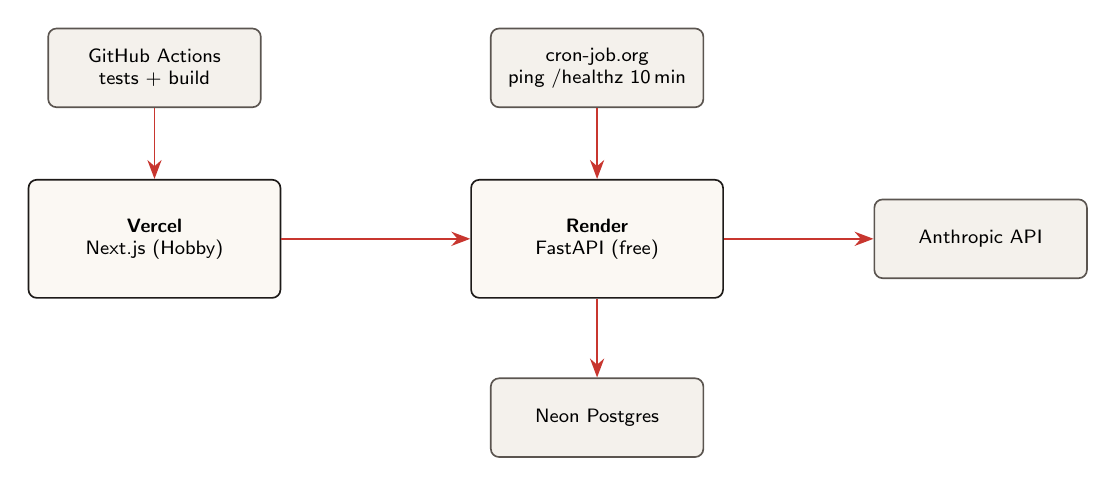
\begin{tikzpicture}[
  font=\sffamily\scriptsize,
  node distance=0.7cm,
  svc/.style={rectangle,rounded corners=3pt,draw=ink,line width=0.6pt,
    fill=paper,minimum width=3.2cm,minimum height=1.5cm,align=center},
  ext/.style={rectangle,rounded corners=3pt,draw=slate,line width=0.6pt,
    fill=codebg,minimum width=2.7cm,minimum height=1.0cm,align=center},
  arr/.style={-{Stealth[length=2.4mm]},line width=0.7pt,color=cinnabar}
]
  \node[svc] (vercel) {\textbf{Vercel}\\\scriptsize Next.js (Hobby)};
  \node[svc,right=2.4cm of vercel] (render) {\textbf{Render}\\\scriptsize FastAPI (free)};
  \node[ext,below=1.0cm of render] (neon) {Neon Postgres};
  \node[ext,above=0.9cm of render] (cron) {cron-job.org\\\scriptsize ping /healthz 10\,min};
  \node[ext,right=1.9cm of render] (claude) {Anthropic API};
  \node[ext,above=0.9cm of vercel] (gh) {GitHub Actions\\\scriptsize tests + build};
  \draw[arr] (vercel)--(render);
  \draw[arr] (render)--(neon);
  \draw[arr] (cron)--(render);
  \draw[arr] (render)--(claude);
  \draw[arr] (gh)--(vercel);
\end{tikzpicture}
\caption{Deployment topology. Every component runs on a free tier; the cron
ping keeps the free Render instance from sleeping.}
\end{figure}

\noindent The entire production stack runs at a recurring cost of
approximately \textbf{\texteuro0}. The only variable cost is Anthropic usage,
bounded by the daily quotas: with prompt caching, a written-expression
correction costs on the order of \$0.003. Infrastructure is declared as code in
\texttt{render.yaml}: the build command, the start command (which applies
pending migrations before serving), the health check and the list of
environment variables, with secrets kept in the hosting dashboard. The front
end redeploys automatically on every push to \texttt{main}; the back end is
redeployed from the Render dashboard.

Operational safeguards, in short: migrations that fail keep the previous
version live; registration can be closed to an allow-list; every Claude call is
metered per user; uploads are bounded (drawings are validated PNGs of at most
1\,MB, 2,000 per user); and text inputs have length limits.

% =============================================================================
\section{Limitations and Next Steps}

\begin{itemize}
  \item \textbf{Exam coverage} --- listening and writing papers cover levels
        1--3; the reading section and levels 4--5 are not reproduced yet. One
        part of the HSK~3.0 level~2 writing paper is listed but unavailable,
        because its official instruction is not published in text.
  \item \textbf{Pictures} --- the pictures of the real papers are replaced by
        written descriptions, which is slightly easier than the exam.
  \item \textbf{Speech} --- voice quality depends on the device; there is no
        speaking practice or pronunciation scoring.
  \item \textbf{Quota reset} --- daily limits reset at midnight UTC rather than
        at the user's local midnight.
  \item \textbf{Answer matching} --- the hanzi-input mode accepts only the
        expected word, not a synonym with the same translation; the learner
        rates the card themselves, which absorbs the ambiguity.
\end{itemize}

% =============================================================================
\section{Conclusion}

HSK Trainer has grown from a vocabulary quiz with an LLM grader into a complete
preparation platform covering vocabulary, listening, writing, grammar,
classifiers, tones and free expression for both versions of the exam. It also
demonstrates a complete path from a quick prototype to a production-shaped
application: a typed, versioned API; a data layer evolved through tested
migrations without losing user progress; reviewed content validated by code; an
LLM integration with structured output, caching, streaming and cost controls;
an optimistic, mobile-first front end; offline test suites with CI; and
zero-cost infrastructure-as-code. The guiding constraint --- that it had to be
a tool worth using daily \emph{and} a credible engineering artefact --- pushed
the design toward explicit, defensible trade-offs rather than defaults. The
result is an application whose every layer can be explained and justified.

\vspace{1.2em}
\noindent{\color{cinnabar}\rule{\linewidth}{1pt}}\\[2pt]
{\sffamily\footnotesize\color{slate}Ivann Vasic \;\textendash\; HSK Trainer \;\textendash\;
FastAPI \textperiodcentered\ Next.js \textperiodcentered\ Postgres \textperiodcentered\ Anthropic Claude}

\end{document}